% DO NOT COMPILE THIS FILE DIRECTLY!
% This is included by the other .tex files.

\begin{frame}
\titlepage
\end{frame}

\begin{frame}
  \frametitle{The aim of this presentation}
  \begin{itemize}
     \item A small update on the state of MISP's ongoing development
     \item Some insight into what new tools we have at our disposal
     \item What can we expect in the coming months
  \end{itemize}
\end{frame}

\begin{frame}
  \frametitle{MISP's evolution since the last MUG}
  \begin{itemize}
    \item Since the last MUG (18/06/2020) we've had:
    \begin{itemize}
        \item 8 releases
        \item 2170 commits
        \item 50 contributors contributing to the core software and its components
    \end{itemize}
  \end{itemize}
\end{frame}

\begin{frame}
  \frametitle{So what were the main changes?}
  \begin{itemize}
     \item The usual {\bf bug- and usability-fixes, quality of life improvements}
     \item Constant internal refactors to prepare us for moving to a more {\bf modern software stack}
     \item Security fixes, including {\bf several CVEs} (keep your MISP up to date!)
     \item Constantly evolving {\bf context libraries and integrations}
     \item Several major features (some that were in development for most of the year)
  \end{itemize}
\end{frame}

\begin{frame}
\frametitle{Event Reports}
\begin{itemize}
	\item MISP's strength has always been {\bf structured information sharing}
        \item {\bf Analyst to Analyst} sharing has been somewhat neglected
        \item The new {\bf Event Report system} aims to address this!
        \item Create {\bf markdown reports} manually...
        \item ...or ingest reports as a starting point
\end{itemize}
\end{frame}

\begin{frame}
\frametitle{Event Reports}
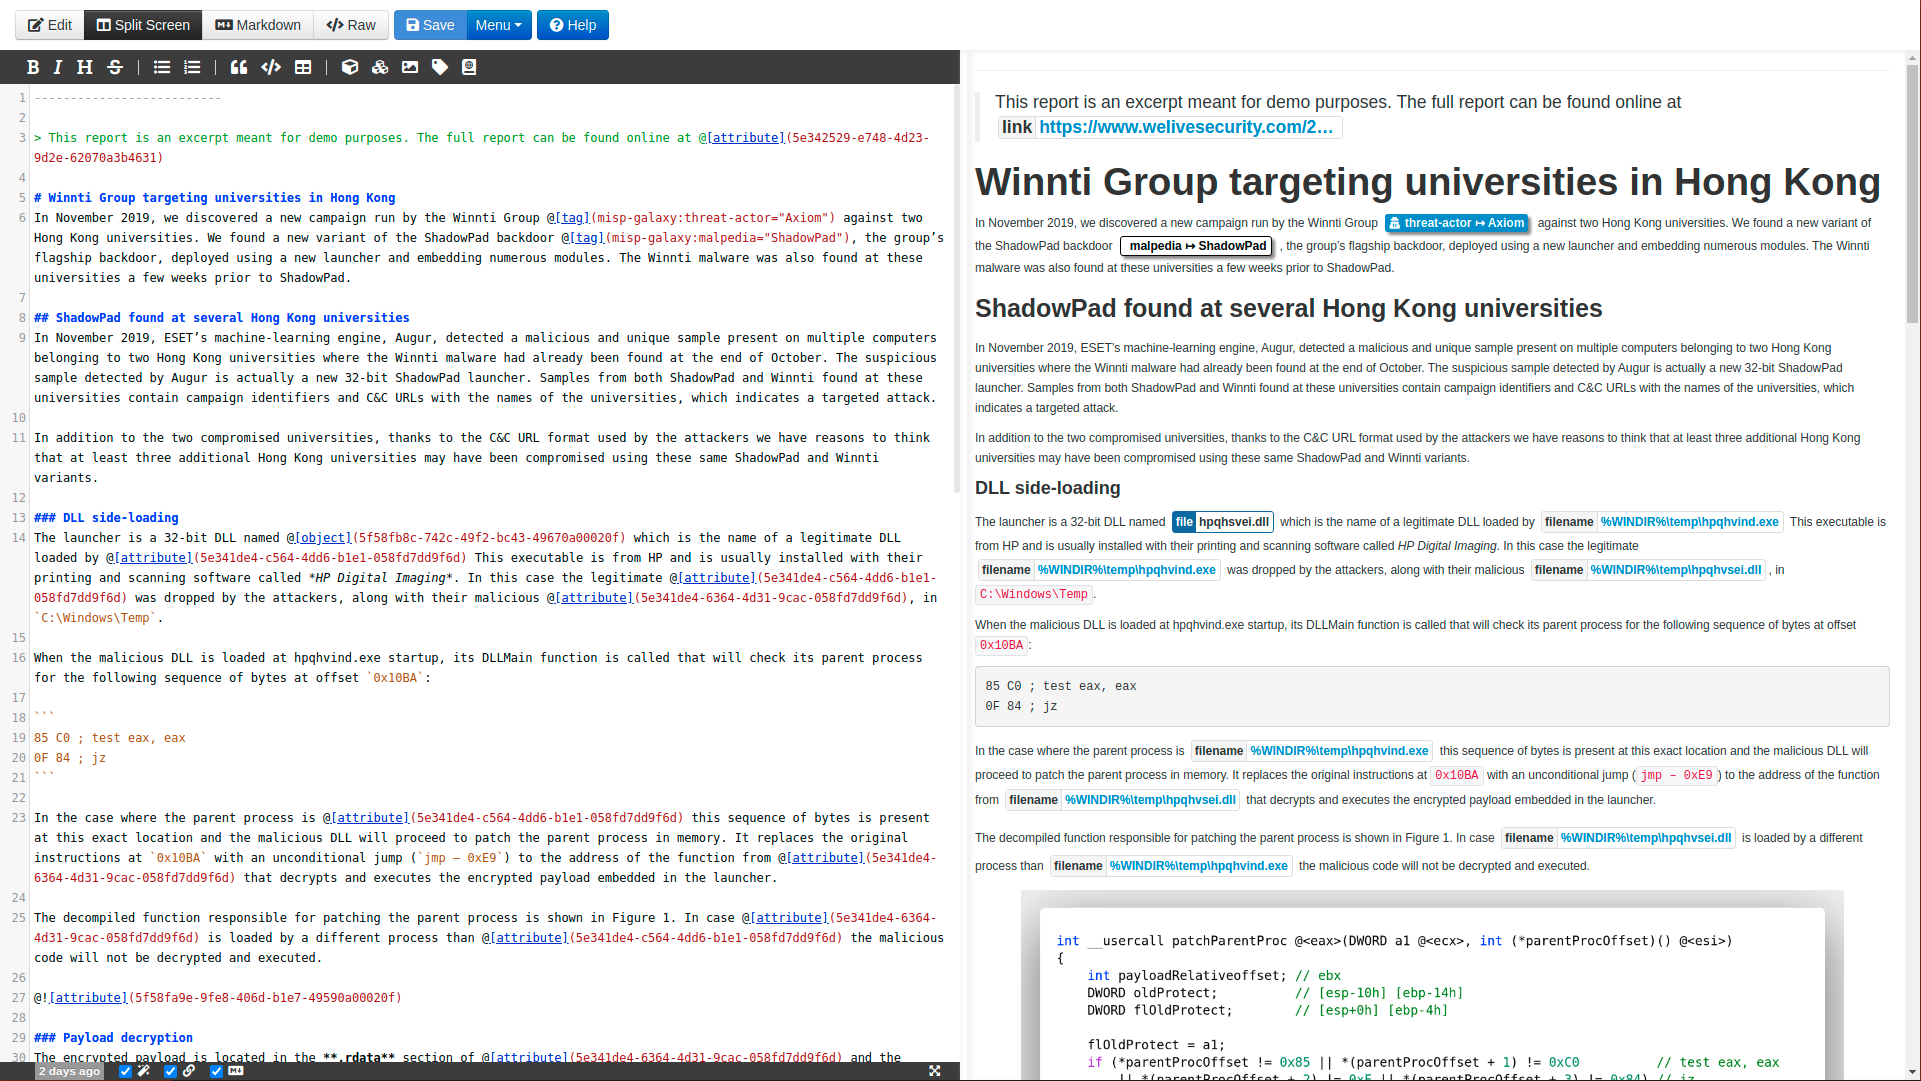
\includegraphics[scale=0.18]{images/eventreport.png}
\end{frame}

\begin{frame}
\frametitle{Event Reports}
\begin{itemize}
	\item Style the text via a live markdown editor
        \item Use custom MISP syntax to {\bf reference MISP attributes/objects}
        \item {\bf Share} the reports along with events
        \item {\bf Restrict the distribution} to subsets of recipients as you would with attributes
        \item Massive toolkit for crafting {\bf complex, rich reports}
\end{itemize}
\end{frame}

\begin{frame}
\frametitle{Galaxy 2.0}
\begin{itemize}
	\item Historically, {\bf higher level contextualisation was quite rigid} in MISP
        \item Galaxies functioned as "tags with extra metadata"
        \item Whilst we could use it to associate our technical data with higher level context...
        \item ...we had no way of redefining the context
        \item We also had no way of encoding our knowledge about how these {\bf concepts were interlinked}
        \item For the past year, our colleague Sami Mokaddem has been working on a solution
\end{itemize}
\end{frame}

\begin{frame}
\frametitle{Galaxy 2.0 - create, modify, fork}
\begin{itemize}
	\item In Galaxy 2.0, in addition to the standard libraries, we introduce the concept of {\bf custom galaxies}
        \item Create {\bf new libraries}, add {\bf new elements} to existing ones, or create {\bf counter-analyses / forks}
        \item Galaxy clusters now follow similar {\bf distribution rules} as all other first class citizens in MISP
\end{itemize}
\noindent\makebox[\textwidth]{%
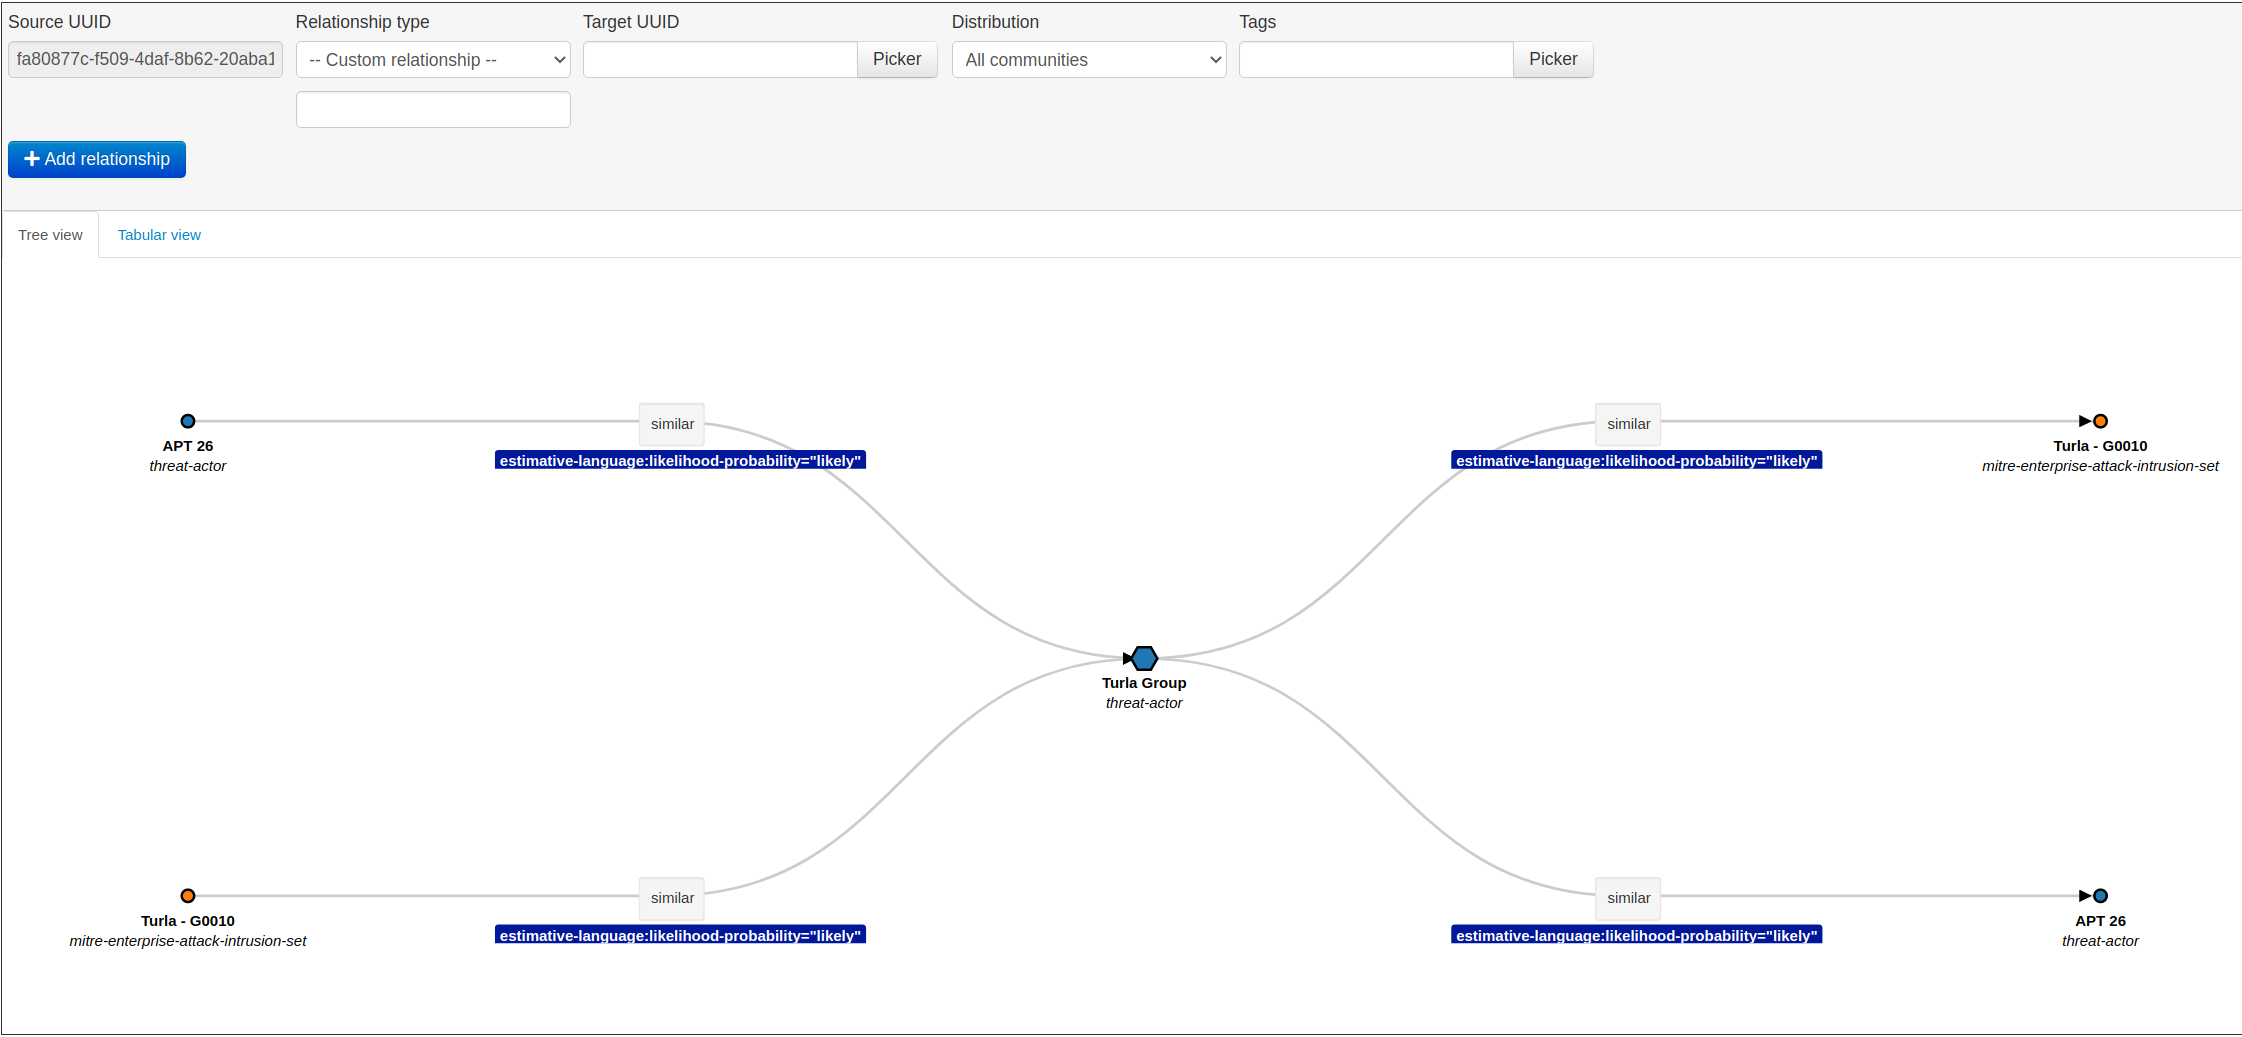
\includegraphics[scale=0.15]{images/galaxy20.png}}
\end{frame}


\begin{frame}
\frametitle{Cerebrate}
\begin{itemize}
	\item A new open-source tool that we're working on
        \item Central component of the {\bf Melicertes} project
        \item {\bf Management and orchestration} tool for communities
        \item Manage {\bf organisations, contact information, sharing groups, tool peering}
        \item First integration with MISP is available already, allows MISP to lookup organisation information
        \item We are launching a {\bf misp-project instance} to centralise organisation uuid management/validation
\end{itemize}
\end{frame}

\begin{frame}
\frametitle{Dashboarding}
\noindent\makebox[\textwidth]{%

\includegraphics[scale=0.19]{images/cerebrate.png}}
\noindent\makebox[\textwidth]{%
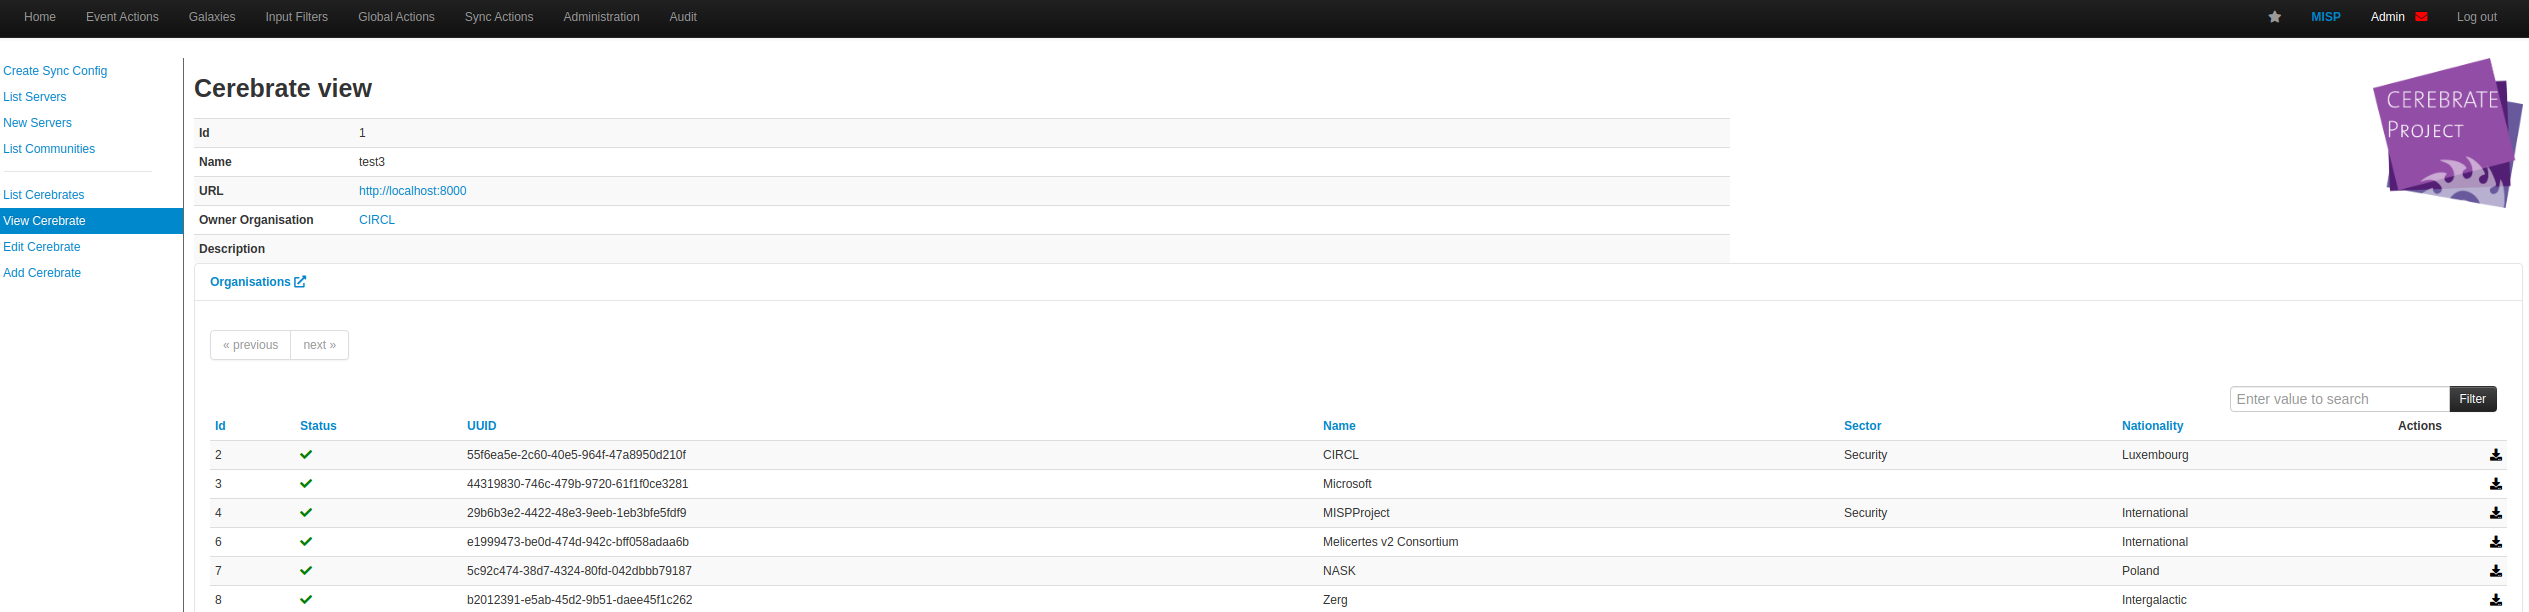
\includegraphics[scale=0.19]{images/mispcerebrate.png}}
\end{frame}

\begin{frame}
\frametitle{Cerebrate}
\begin{itemize}
	\item In the future we'll expand the use-cases and integrations with MISP
        \item Ease the {\bf interconnection of MISPs} for synchronisation
        \item Manage {\bf MISPs and MISP users} for organisations with multiple MISPs
        \item Lookup system for public keys for {\bf information veracity validation}
\end{itemize}
\end{frame}

\begin{frame}
\frametitle{New API key system}
\begin{itemize}
	\item {\bf On-demand} functionality
        \item Stores API keys hashed
        \item {\bf Multiple keys per user} account
        \item Individual {\bf expiration} and {\bf descriptions} for the API keys
        \item Tooling for a painless transition to the modern API key system
\end{itemize}
\noindent\makebox[\textwidth]{%
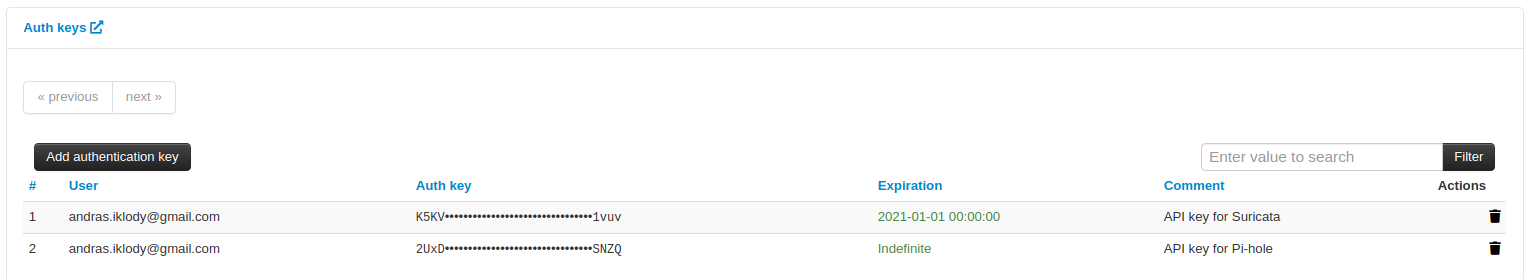
\includegraphics[scale=0.32]{images/authkey.png}}
\end{frame}

\begin{frame}
\frametitle{Interoperability}
\begin{itemize}
	\item Constant co-operation with vendors
        \item We've had several new integrations contributed by 3rd parties and developed in-house
        \item Several more integrations in the pipe, both with proprietary and OSS tools
        \item New integrations are supporting the {\bf rich MISP standard format} going beyond simple IoC sharing
        \begin{itemize}
            \item Some notable ones: Intel 471 MISP feeds, Farsight dnsdb 2 misp-modules, etc
        \end{itemize}
        \item Constant improvements for {\bf standard specific} integrations (such as STIX 2.1)
        \item Collaboration with other CSIRTs on building a larger {\bf eco-system of OSS tools} (Melicertes)
\end{itemize}
\end{frame}

\begin{frame}
\frametitle{Knowledge base and classification libraries}
\begin{itemize}
	\item Constant flow of new libraries and improvements
        \item Many topical libraries, some examples:
        \begin{itemize}
            \item China Defence Universities Tracker
            \item SoD-Matrix (Segregation (or separation) of Duties (SoD) Matrix for CSIRTs, LEA and Judiciary)
        \end{itemize}
	\item ATT\&CK sub-techniques have been mapped (Thanks to Christophe Vandeplas!)
\end{itemize}
\end{frame}

\begin{frame}
\frametitle{SoD matrix example}
\begin{itemize}
	\item Describe domain specific libraries using the ATT\&CK methodology
        \item Lends itself to a lot of different use-cases
\end{itemize}
\noindent\makebox[\textwidth]{%
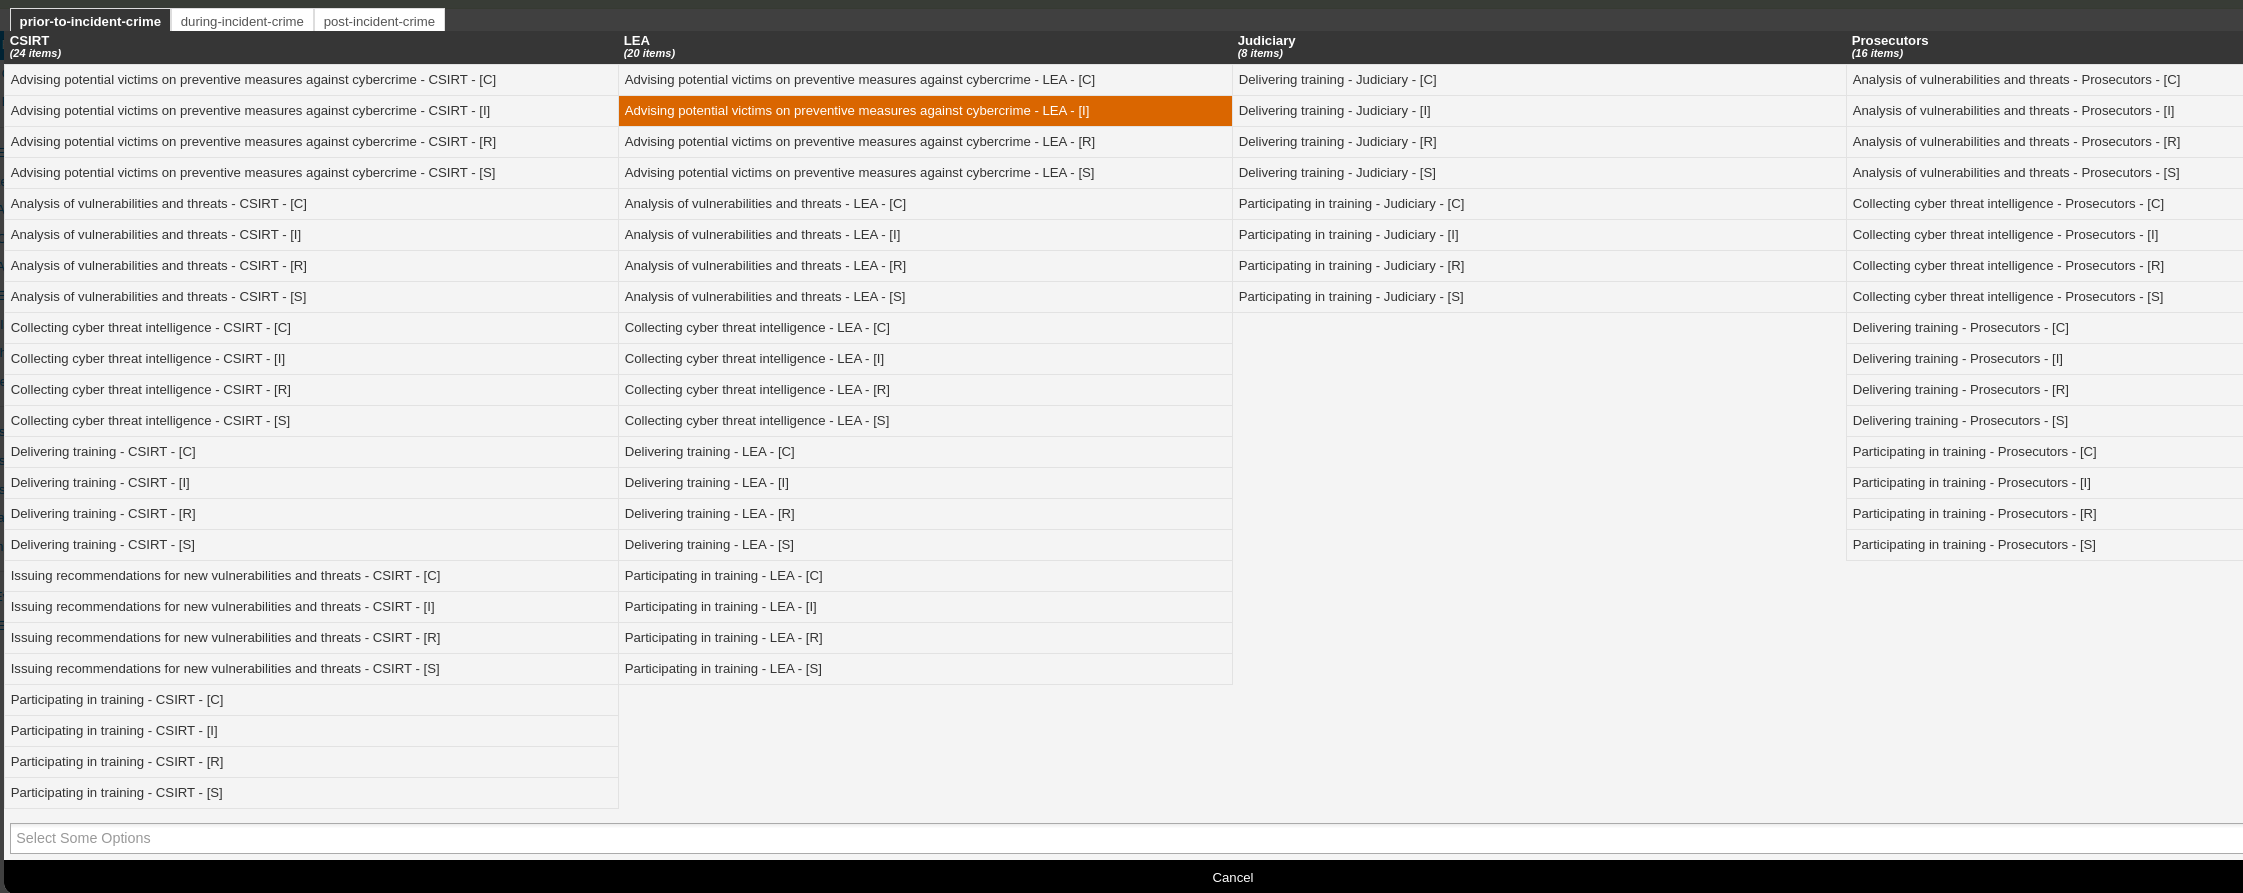
\includegraphics[scale=0.21]{images/SoD.png}}
\end{frame}

\begin{frame}
\frametitle{What's in the pipe?}
\begin{itemize}
	\item Long overdue move to a more {\bf modern stack} - in progress behind the scenes for a while
        \item Cerebrate also acts as our playground for the modern stack
        \item Larger focus on {\bf community management}
        \item Cryptographic {\bf signing of data}
        \item MISP over the past 2 years has heavily shifted focus to also include higher level threat intel sharing
        \item Even though we now have the systems in place, we expect to capitalise on and improve these features heavily
        \item {\bf New release pipeline} that we've switched to right now (to accomodate the additional testing)
\end{itemize}
\end{frame}

\begin{frame}
  \frametitle{To sum it all up...}
  \begin{itemize}
     \item The MISP {\bf developer community is constantly growing} and improvements are coming in at a crazy rate
     \item We have {\bf wrapped up several longer projects} that have been underway for over a year recently
     \item The main focus this year has been {\bf fleshing out threat intelligence and contextual} information sharing
     \item As well as {\bf community management} to tackle our growing and more interconnected community networks
     \item We have more ideas than can be implemented with days only having 24 hours, there are {\bf many ways to get involved}
     \item Prioritisation is hard. {\bf Let us know what you think we should focus on}!
  \end{itemize}
\end{frame}

\begin{frame}
  \frametitle{Get in touch if you have any questions}
  \begin{itemize}
    \item Contact CIRCL
    \begin{itemize}
      \item info@circl.lu
      \item \url{https://twitter.com/circl_lu}
      \item \url{https://www.circl.lu/}
    \end{itemize}
    \item Contact MISPProject 
    \begin{itemize}
      \item \url{https://github.com/MISP}
      \item \url{https://gitter.im/MISP/MISP}
      \item \url{https://twitter.com/MISPProject}
    \end{itemize}
    \item Cerebrate project
    \begin{itemize}
      \item \url{https://github.com/cerebrate-project}
      \item \url{https://github.com/cerebrate-project/cerebrate}
    \end{itemize}
    \item Join the COVID-19 MISP community
    \begin{itemize}
      \item \url{https://covid-19.iglocska.eu}
    \end{itemize}
  \end{itemize}
\end{frame}
